We now turn to discuss how different predictions compare when the matching to parton-shower (PS) is included. For such
a comparison we expect larger discrepancy than what we found at fixed-order, as a consequence of the different
matching schemes, PS employed and of the other details of the matching (such as the choice of the shower initial scale). Among
the codes capable of providing fixed-order results, presented before, {\sc MG5\_aMC}, {\sc POWHEG} and {\sc VBFNLO}
can also provide results at (N)LO+PS accuracy. Besides, also {\sc PHANTOM} is employed for LO+PS results.\\
{\sc MG5\_aMC},
which
employs the {\sc MC@NLO}~\cite{Frixione:2002ik} matching procedure, will be used together with {\sc Pythia8}~\cite{Sjostrand:2014zea} (version 2.2.3) 
and {\sc Herwig++}~\cite{Bahr:2008pv, Bellm:2013hwb} (version 2.7.1). For {\sc POWHEG}, the omonymous matching procedure is 
employed~\cite{Nason:2004rx,Frixione:2007vw}, together with {\sc Pythia8} 
{\bf MZ VERSION? if same as MG5, put it at the end together with the tune}. {\sc VBFNLO} makes it possible to choose between the {\sc MC@NLO} and {\sc POWHEG}
matching, in both cases together with {\sc Herwig7}~\cite{}. Finally, {\sc PHANTOM} results will be shown matched with {\sc Pythia 8}.
Whenever {\sc Pythia8}\ is used, the Monash tune~\cite{Skands:2014pea} is selected.\\

Results will be presented within the cuts described in Section~\ref{subsec:inputpar}, applied after shower and hadronization (this implies that jets
are obtained by clustering stable hadrons, and not QCD partons). This implies that at the event-generation level, looser cuts (or no cuts at all) 
must be emplouyed in order not to bias the results. {\bf MZ lepton-jet separation at the hard-event level?}.\\

A slightly different setup has been employed for {\sc MG5\_aMC} in order to simplify the calculation: instead of generating the full 
${\rm p}{\rm p}\to\mu^+\nu_\mu{\rm e}^+\nu_{\rm e}{\rm j}{\rm j}$ process, since it is anyway dominated by doubly-resonant contribution, the 
events are produced for the process with two stable W$^+$ bosons (${\rm p}{\rm p}\to{\rm W^+}{\rm W^+}{\rm j}{\rm j}$), and these W$^+$ bosons
are decayed with {\sc MadSpin}~\cite{Artoisenet:2012st} (keeping spin correlations) before the PS. Since {\sc MadSpin}\ computes 
the partial and total decay width of the W bosons at LO accuracy only, while in Section~\ref{subsec:inputpar} the NLO width is employed, 
a small effect (6\%) on the normalisation of distribution is induced. Finally, when the renormalisation
and factorisation scales are set, the $\Delta R_{\Pj\Pl}$ cut is not imposed during the jet-clustering procedure, but this has no visible effect 
on the results.

We now turn to present the results:



\begin{table}[h!]
    \centering
    \begin{tabular}{c|c|c|c}
        Code  &  $\sigma[\rm{fb}]$  \\
        \hline
        {\sc MG5\_aMC}+{\sc Pythia8}&  $1.450 (1.368) \pm 0.$  \\
        {\sc MG5\_aMC}+{\sc Herwig++}&  $1.445 (1.363) \pm 0.$  \\
        {\sc POWHEG}  &  $1.3633 \pm 0.0004$  \\
        {\sc VBFNLO}  &  $X \pm 0.0003$  \\
        \hline
        {\sc MG5\_aMC}+{\sc Pythia8} (LO)&  $1.352 (1.275) \pm 0.$  \\
        {\sc MG5\_aMC}+{\sc Herwig++} (LO)&  $X  \pm 0.$  \\
        {\sc PHANTOM} &  $1.235  \pm 0.$  \\
    \end{tabular}
    \caption{\label{tab:wg1_NLOrates} Rates at NLO-QCD (LO-QCD) accuracy matched to parton shower within VBS cuts obtained with the different codes used in this comparison, 
    for the ${\rm p}{\rm p}\to\mu^+\nu_\mu{\rm e}^+\nu_{\rm e}{\rm j}{\rm j}$ process. Numbers in parentheses for the {\sc MG5\_aMC} simulations
    are rescaled to account for the effect related to the boson widths computed by {\sc MadSpin}, see the text for details.}
{\bf MZ: MC uncertainties???}
\end{table}

\begin{figure*}[hbt]
\centering
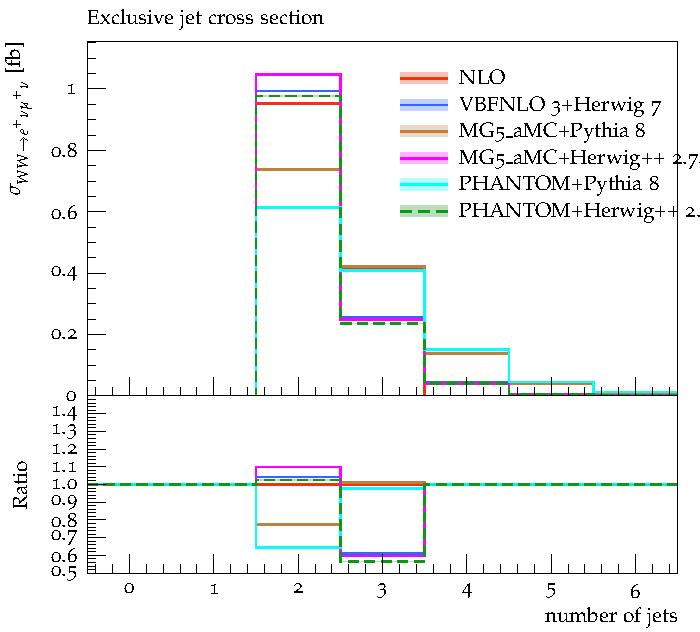
\includegraphics[width=0.47\textwidth]{figures/LOPS/jetsexclusive.pdf}
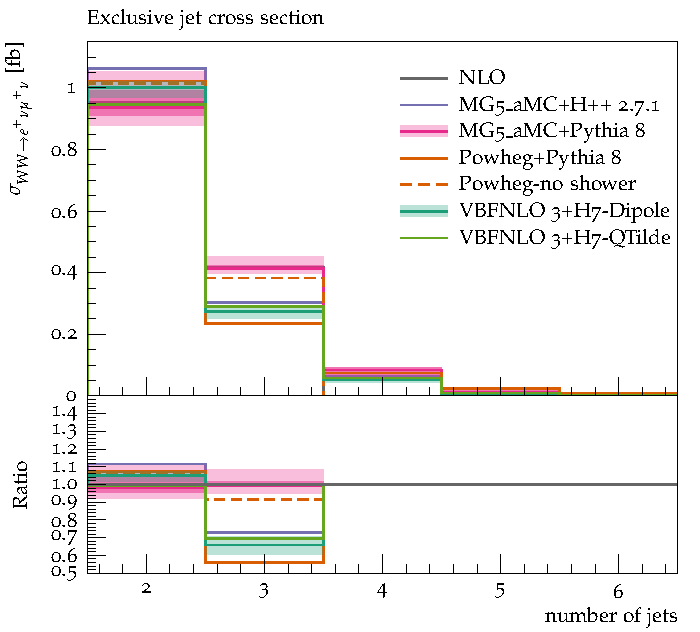
\includegraphics[width=0.47\textwidth]{figures/NLOPS/jetsexclusive.pdf}
\caption{Exclusive jet multiplicity from predictions matched to parton shower, at LO (left) or NLO (right) accuracy, compared with the fixed-NLO result
    computed with \sc{VBFNLO}}
\label{fig:PSnjet}
\end{figure*}

\begin{figure*}[hbt]
\centering
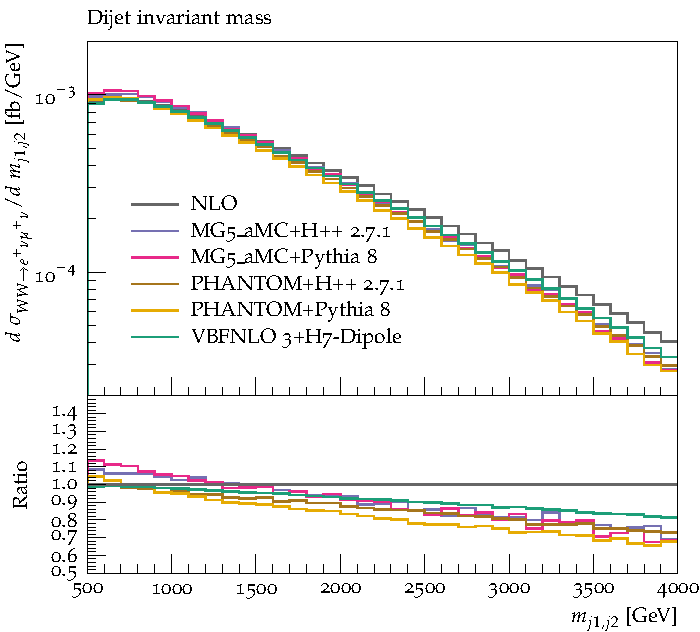
\includegraphics[width=0.47\textwidth]{figures/LOPS/m_jj.pdf}
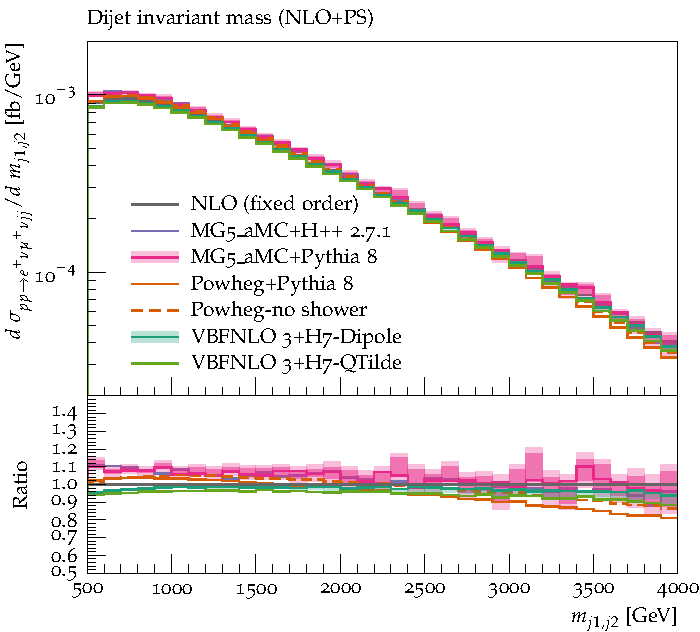
\includegraphics[width=0.47\textwidth]{figures/NLOPS/m_jj.pdf}
\caption{Same as in Fig.~\protect\ref{fig:PSnjet}, for the invariant mass of the two tagging jets.}
\label{fig:PSmjj}
\end{figure*}

\begin{figure*}[hbt]
\centering
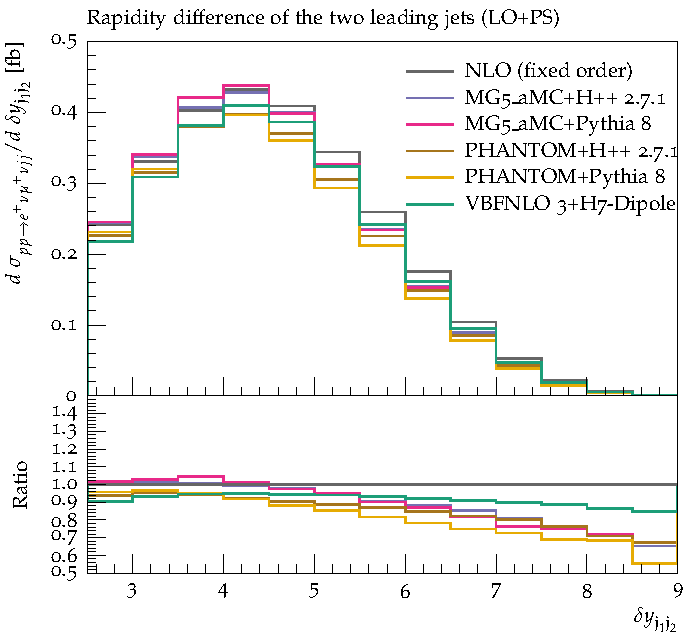
\includegraphics[width=0.47\textwidth]{figures/LOPS/Deltay_jj.pdf}
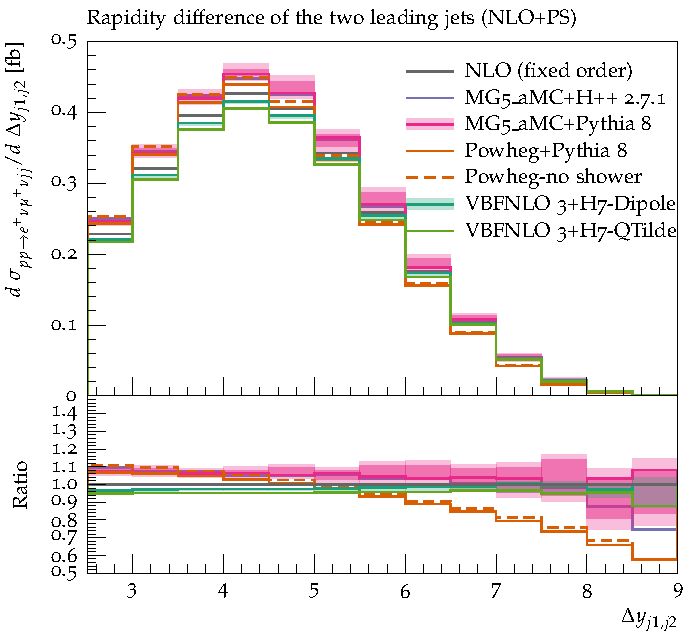
\includegraphics[width=0.47\textwidth]{figures/NLOPS/Deltay_jj.pdf}
\caption{Same as in Fig.~\protect\ref{fig:PSnjet}, for the rapidity separation of the two tagging jets.}
\label{fig:PSdyjj}
\end{figure*}

\begin{figure*}[hbt]
\centering
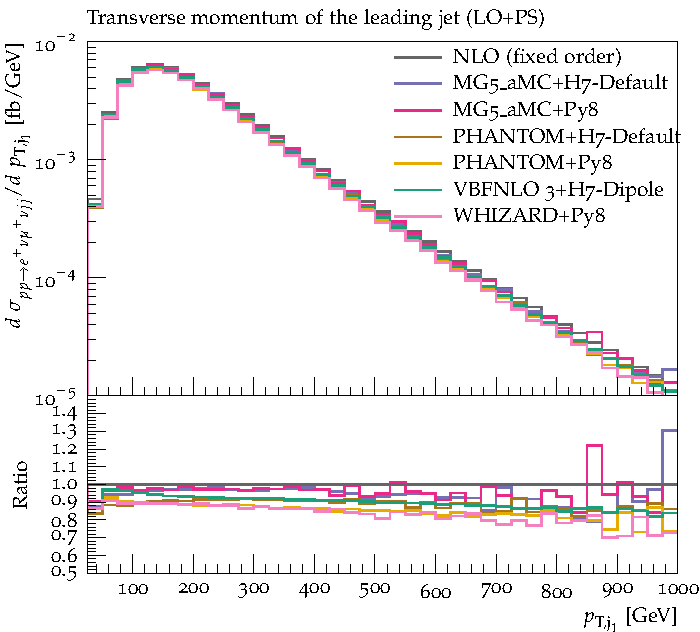
\includegraphics[width=0.47\textwidth]{figures/LOPS/pT_j1.pdf}
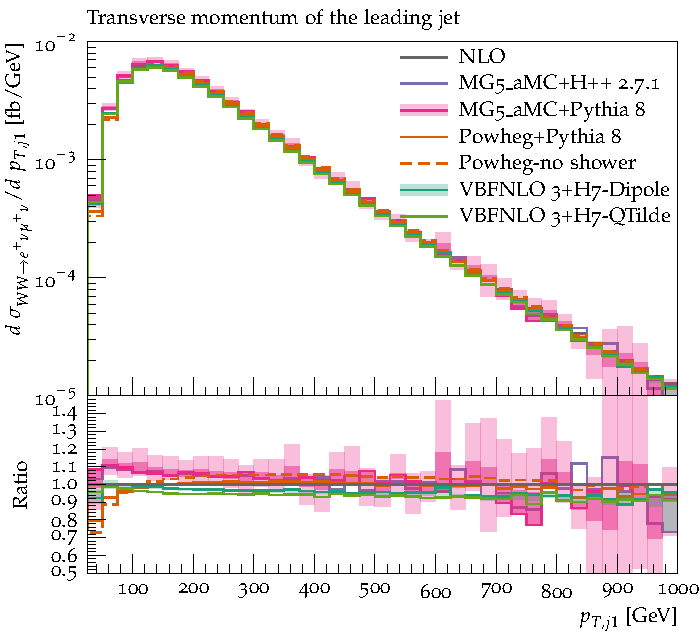
\includegraphics[width=0.47\textwidth]{figures/NLOPS/pT_j1.pdf}
\caption{Same as in Fig.~\protect\ref{fig:PSnjet}, for the invariant mass of the two tagging jets.}
\label{fig:PSpt1}
\end{figure*}

\begin{figure*}[hbt]
\centering
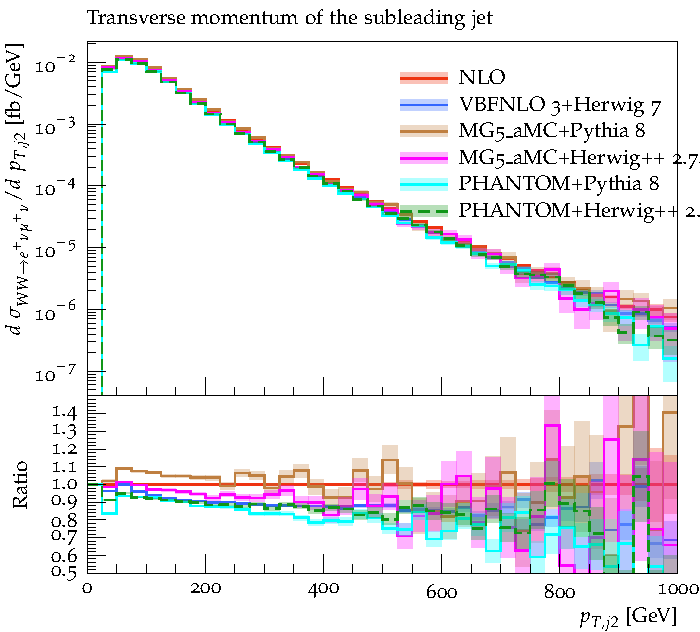
\includegraphics[width=0.47\textwidth]{figures/LOPS/pT_j2.pdf}
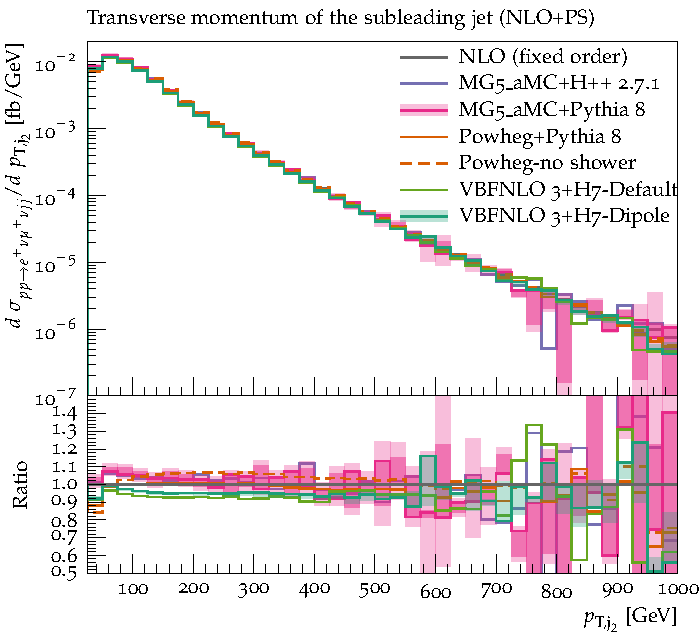
\includegraphics[width=0.47\textwidth]{figures/NLOPS/pT_j2.pdf}
\caption{Same as in Fig.~\protect\ref{fig:PSnjet}, for the invariant mass of the two tagging jets.}
\label{fig:PSpt2}
\end{figure*}

\begin{figure*}[hbt]
\centering
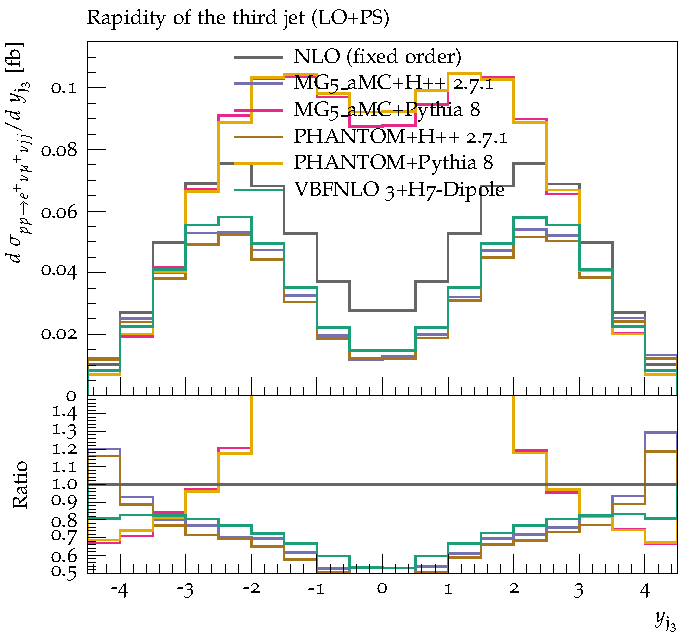
\includegraphics[width=0.47\textwidth]{figures/LOPS/y_j3.pdf}
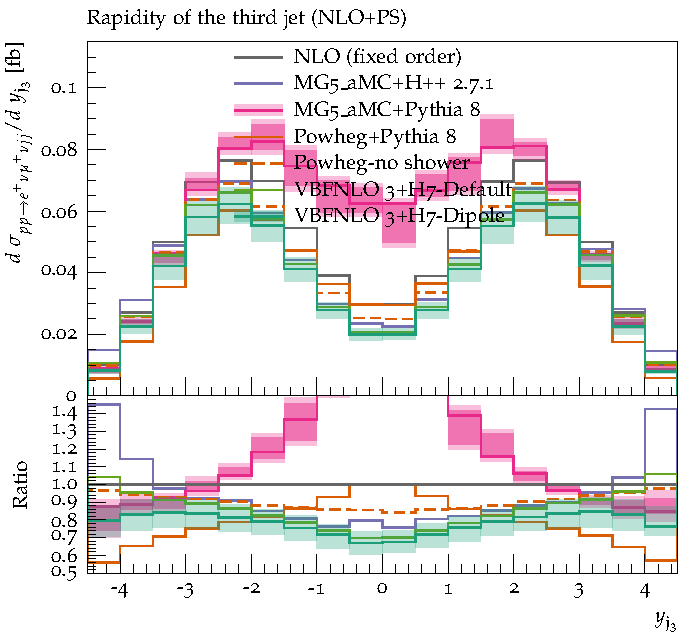
\includegraphics[width=0.47\textwidth]{figures/NLOPS/y_j3.pdf}
\caption{Same as in Fig.~\protect\ref{fig:PSnjet}, for the invariant mass of the two tagging jets.}
\label{fig:PSy3}
\end{figure*}
